%------------------------------------------------------------------------------
% CV in Latex
% Author : Charles Rambo
% Based off of: https://github.com/sb2nov/resume and Jake's Resume on Overleaf
% Most recently updated version may be found at https://github.com/fizixmastr 
% License : MIT
%------------------------------------------------------------------------------

\documentclass[A4,11pt]{article}
%\documentclass[letterpaper,11pt]{article} %For use in US
\usepackage{latexsym}
\usepackage[empty]{fullpage}
\usepackage{titlesec}
\usepackage{marvosym}
\usepackage[usenames,dvipsnames]{color}
\usepackage{verbatim}
\usepackage{enumitem}
\usepackage[hidelinks]{hyperref}
\usepackage[english]{babel}
\usepackage{tabularx}
\usepackage{tikz}

\hypersetup{
	colorlinks   = true,
	citecolor    = black!60
}


\begin{comment}
	I am by no means a professional when it comes to the CV's/resumes, I have
	received various trainings on how to write a CV and resume from my high 
	school, as well as the Austin College and University of Eastern Finland's
	career counseling departments. As I intend to share my CV as a template, I 
	feel that it is my responsibility to provide explanations of my work.
\end{comment}


%-----FONT OPTIONS-------------------------------------------------------------
\begin{comment}
	The font of the document will impact not just how readable it is, but how it is
	perceived. In the "The Craft of Scientific Writing" by Michael Alley, shares a
	common fonts for publication as well as their use. I have chosen to use
	Palatino for its legibility, some others are given below. There is far too much
	about typography to discus here. Note: serif fonts have short projecting
	strokes, sans-serif fonts are sans (without) these strokes.
\end{comment}


% serif
\usepackage{palatino}
% \usepackage{times} %This is the default as well
% \usepackage{charter}

% sans-serif
% \usepackage{helvet}
% \usepackage[sfdefault]{noto-sans}
% \usepackage[default]{sourcesanspro}

%-----PAGE SETUP---------------------------------------------------------------

% Adjust margins
\addtolength{\oddsidemargin}{-1cm}
\addtolength{\evensidemargin}{-1cm}
\addtolength{\textwidth}{2cm}
\addtolength{\topmargin}{-1cm}
\addtolength{\textheight}{2cm}

% Margins for US Letter size
%\addtolength{\oddsidemargin}{-0.5in}
%\addtolength{\evensidemargin}{-0.5in}
%\addtolength{\textwidth}{1in}
%\addtolength{\topmargin}{-.5in}
%\addtolength{\textheight}{1.0in}

\urlstyle{same}

\raggedbottom
\raggedright
\setlength{\tabcolsep}{0cm}

% Sections formatting
\titleformat{\section}{
	\vspace{-4pt}\scshape\raggedright\large
}{}{0em}{}[\color{black}\titlerule \vspace{-5pt}]

% Ensure that .pdf is machine readable/ATS parsable
\pdfgentounicode=1

%-----CUSTOM COMMANDS FOR FORMATTING SECTIONS----------------------------------
\newcommand{\CVItem}[1]{
	\item\small{
		{#1 \vspace{-2pt}}
	}
}

\newcommand{\CVRubheading}[3]{
	\vspace{-2pt}\item
	\textbf{#1}
	\begin{tabular*}{0.97\textwidth}[t]{l@{\extracolsep{\fill}}r}
		\small#2 & \small #3 \\
	\end{tabular*}\vspace{-7pt}
}

\newcommand{\CVSubheading}[4]{
	\vspace{-2pt}\item
	\begin{tabular*}{0.97\textwidth}[t]{l@{\extracolsep{\fill}}r}
		\textbf{#1} & #2 \\
		\small#3 & \small #4 \\
	\end{tabular*}\vspace{-7pt}
}

\newcommand{\CVTubheading}[7]{
	\vspace{0pt}\item
	\begin{tabular*}{0.97\textwidth}[t]{l@{\extracolsep{\fill}}r}
		\textbf{#1} & #2 \\
		\small#3 & \small #4 \\
		\small#5 & \small #6 \\
	\end{tabular*}
	{\small $\rhd$ #7} \vspace{0pt}
}

\newcommand{\CVSubSubheading}[2]{
	\item
	\begin{tabular*}{0.97\textwidth}{l@{\extracolsep{\fill}}r}
		\text{\small#1} & \text{\small #2} \\
	\end{tabular*}\vspace{-7pt}
}

\newcommand{\CVSubItem}[1]{\CVItem{#1}\vspace{-4pt}}

\renewcommand\labelitemii{$\vcenter{\hbox{\tiny$\bullet$}}$}

\newcommand{\CVSubHeadingListStart}{\begin{itemize}[leftmargin=0.5cm, label={}]}
	% \newcommand{\resumeSubHeadingListStart}{\begin{itemize}[leftmargin=0.15in, label={}]} % Uncomment for US
		\newcommand{\CVSubHeadingListEnd}{\end{itemize}}
	\newcommand{\CVItemListStart}{\begin{itemize}}
		\newcommand{\CVItemListEnd}{\end{itemize}\vspace{-5pt}}
	
	%------------------------------------------------------------------------------
	% CV STARTS HERE  %
	%------------------------------------------------------------------------------
	\begin{document}
		
		%-----HEADING------------------------------------------------------------------
		\begin{comment}
			In Europe it is common to include a picture of ones self in the CV. Select
			which heading appropriate for the document you are creating.
		\end{comment}
		
		\begin{minipage}[c]{0.05\textwidth}
			\-\
		\end{minipage}
		\begin{minipage}[c]{0.2\textwidth}
			\begin{tikzpicture}
				\clip (0,0) circle (1.75cm);
				\node at (0,-0.1) {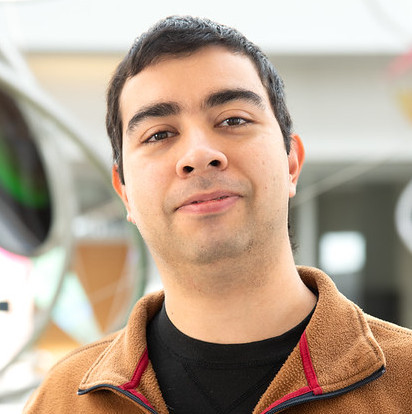
\includegraphics[width = 4cm]{53500746199_4b98a4c178_c.jpg}}; 
				% if necessary the picture may be moved by changing the at (coordinates)
				% width defines the 'zoom' of the picture
			\end{tikzpicture}
			\hfill\vline\hfill
		\end{minipage}
		\begin{minipage}[c]{0.4\textwidth}
			\textbf{\Huge \scshape{Erik Am\'ezquita}} \\ \vspace{1pt} 
			% \scshape sets small capital letters, remove if desired
			\small{+1 517-755-8202} \\
			\href{mailto:eah4d@missouri.edu}{\underline{eah4d@missouri.edu}}\\
			% Be sure to use a professional *personal* email address
			\href{https://www.linkedin.com/in/erik-amezquita/}{\underline{linkedin.com/in/erik-amezquita/}} \\
			% you should adjust you linked in profile name to be professional and recognizable
			\href{https://ejamezquita.github.io/}{\underline{ejamezquita.github.io/}}
		\end{minipage}
		\begin{minipage}[c]{0.3\textwidth}
			\vspace{1.5em}
			\small{1201 Rollins St\\371h Bond Life Sciences Center\\Columbia, MO 65211\\USA}
		\end{minipage}
		
		% Without picture
		%\begin{center}
		%    \textbf{\Huge \scshape Charles Rambo} \\ \vspace{1pt} %\scshape sets small capital letters, remove if desired
		%    \small +1 123-456-7890 $|$ 
		%    \href{mailto:you@provider.com}{\underline{you@provider.com}} $|$\\
		%    % Be sure to use a professional *personal* email address
		%    \href{https://linkedin.com/in/your-name-here}{\underline{linkedin.com/in/charles-rambo}} $|$
		%    % you should adjust you linked in profile name to be professional and recognizable
		%    \href{https://github.com/fizixmastr}{\underline{github.com/fizixmastr}}
		%\end{center}
		
		
		
		\begin{comment}
			This CV was written for specifically for positions I was applying for in
			academia, and then modified to be a template.
			
			A standard CV is about two pages long where as a resume in the US is one page.
			sections can be added and removed here with this in mind. In my experience, 
			education, and applicable work experience and skills are the most import things
			to include on a resume. For a CV the Europass CV suggests the categories: Work
			Experience, Education and Training, Language Skills, Digital Skills,
			Communication and Interpersonal Skills, Conferences and Seminars, Creative Works
			Driver's License, Hobbies and Interests, Honors and Awards, Management and
			Leadership Skills, Networks and Memberships, Organizational Skills, Projects,
			Publications, Recommendations, Social and Political Activities, Volunteering.
			
			Your goal is to convey a who, what , when, where, why for every item you share. 
			The who is obviously you, but I believe the rest should be done in that order.
			For example below. An employer cares most about the degree held and typically 
			less about the institution or where it is located (This is still good 
			information though). Whatever order you choose be consistent throughout.
		\end{comment}
		
		%-----EDUCATION----------------------------------------------------------------
		\section{Empleo y Educaci\'on}
		\CVSubHeadingListStart
		%    \CVSubheading % Example
		%      {Degree Achieved}{Years of Study}
		%      {Institution of Study}{Where it is located}
		\CVSubheading
		{{Investigador Posdoctoral $|$ \emph{\small{Biolog\'ia Vegetal (80\%) y Matem\'aticas (20\%)}}}}{Jul.~2023 -- presente}
		{Division of Plant Science \& Technology, University of Missouri}{Columbia, Missouri, EEUU}
		\CVTubheading
		{{Doctorado (PhD) $|$ \emph{\small{C\'omputo Matem\'atico Cient\'ifico e Ingenier\'ia}}}}{Ago.~2018 -- Mayo 2023}
		{Computational Mathematics, Science \& Engineering, Michigan State University}{East Lansing, Michigan, EEUU}
		{Tesis: \emph{Exploring the Mathematical Shape of Plants}}{Promedio: 4.0/4.0}{Premio Fitch H. Beach 2022 a la mejor investigaci\'on de posgrado en la Facultad de Ingenieria de la Universidad}
		\CVTubheading
		{{Licenciatura $|$ \emph{\small{Matem\'aticas}}}}{Ago.~2013 -- Jun.~2018}
		{Departamento de Matem\'aticas, Universidad de Guanajuato}{Guanajuato, Guanajuato, M\'exico}
		{Tesis: \emph{Efficient object classification using the Euler Characteristic}}{Promedio: 9.85/10}{Premio Sotero Prieto 2018 a la Mejor Tesis de Licenciatura en Matem\'aticas en M\'exico}
		\CVSubHeadingListEnd
		
		%-----WORK EXPERIENCE----------------------------------------------------------
		\begin{comment}
			try to briefly explain what you did and why it is relevant to the position you
			are seeking
		\end{comment}
		
		\section{Proyectos desarrollados y Experiencia en Investigaci\'on Relevantes}
		\CVSubHeadingListStart
		%    \CVSubheading %Example
		%      {What you did}{When you worked there}
		%      {Who you worked for}{Where they are located}
		%      \CVItemListStart
		%        \CVItem{Why it is important to this employer}
		%      \CVItemListEnd
		\CVRubheading
		{Modelado matem\'atico de patrones y distribuciones espaciales transcritos de ARNm a nivel subcelular}
		{Division of Plant Science \& Technology, University of Missouri}{Oct.~2023 -- presente}
		\CVItemListStart
		\CVItem{Caracterizaci\'on matem\'atica de transcritos de ARNm dentro de c\'elulas de la ra\'iz de soya (\emph{Glycine max})}
		\CVItem{Uso de Python y An\'alisis Tol\'ogico de Datos para el modelado de patrones espaciales celulares}
		%\CVItem{Identificaci\'on de patrones distintivos de ARNm en c\'elulas senescentes para diversos genes}
		%\CVItem{An\'alisis desarrollado en Python con posibilidad de adaptar a m\'as datos transcript\'omicos espaciales}
		\CVItemListEnd
		\CVRubheading
		{Fenotipado autom\'atico del movimiento de \emph{Cuscuta campestris} con seguimiento de objetos}
		{Division of Plant Science \& Technology, University of Missouri}{Jul.~2023 -- Abril 2024}
		\CVItemListStart
		\CVItem{Uso de Python para detectar el movimiento de \emph{Cuscuta} a medida que \'esta se enrolla en posibles hu\'espedes}
		\CVItem{Identificaci\'on autom\'atica de tiempos y velocidades de enroscamiento dependientes de la hora del d\'ia}
		\CVItemListEnd
		\CVRubheading
		{An\'alisis matem\'atico de morfolog\'ia de nueces con tomograf\'ias 3D}
		{Division of Plant Science \& Technology, University of Missouri}{Oct.~2022 -- Dic.~2023}
		\CVItemListStart
		\CVItem{Uso de Python para analizar tomograf\'ias 3D y calcular 50 fenotipos morfol\'ogicos de nueces (\emph{Juglans regia})}
		\CVItem{Determinaci\'on de los 4 fenotipos morfol\'ogicos m\'as predictivos de caracter\'isticas de interes comercial}
		\CVItemListEnd
		\CVRubheading
		{An\'alisis de datos gen\'omicos a trav\'es de topolog\'ia algebraica aplicada}
		{Computational Mathematics, Science \& Engineering, Michigan State University}{Ene.~2020 -- Mar.~2023}
		\CVItemListStart
		\CVItem{Reducci\'on de dimensi\'on y clusterizaci\'on de perfiles gen\'eticos de tejido pulmonar sano y cancer\'igeno}
		\CVItem{Detecci\'on de subtipos de cancer pulmonar previamente no identificados}
		\CVItemListEnd
		\CVRubheading
		{Modelado estad\'istico de la distribuci\'on de gl\'andulas de aceite en c\'itricos}
		{Computational Mathematics, Science \& Engineering, Michigan State University}{Oct.~2021 -- Dic.~2022}
		\CVItemListStart
		\CVItem{Desarrollo de software en Python para analizar tomograf\'ias 3D de c\'itricos y aislar sus gl\'andulas de aceite}
		\CVItem{Uso de estad\'istica direccional para modelar la distribuci\'on de las gl\'andulas a lo largo de la c\'ascara de la fruta}
		\CVItemListEnd
		\CVRubheading
		{Caracterizaci\'on matem\'atica de la morfolog\'ia de granos de cebada}
		{Computational Mathematics, Science \& Engineering, Michigan State University}{Ago.~2019 -- Dic.~2021}
		\CVItemListStart
		\CVItem{Desarrollo de software en Python para analiza tomograf\'ias 3D de espigas de cebada (\emph{Hordeum vulgare})}
		\CVItem{Uso de aprendizaje de m\'aquina (ML) para predecir el genotipo de la semilla basado solo en su morfolog\'ia}
		\CVItemListEnd
		\CVSubHeadingListEnd
		
		
		\section{Habilidades generales}
		\begin{itemize}[leftmargin=0.5cm, label={}]
			\small{\item{
					\textbf{Idiomas}{: Espa\~nol (nativo), Ingl\'es (pr\'acticamente nativo), Franc\'es (elemental)} \\
					\textbf{Programaci\'on}{: Python (NumPy, SciPy, Pandas, Scikit-Learn, Scikit-Image), R (tidyverse), C/C++, bash/unix} \\
					\textbf{Tecnolog\'ias}{: \LaTeX, RMarkdown, Jupyter, vim, html/css} \\
			}}
		\end{itemize}
		
		%------------------------------------------------------------------------------
	\end{document}